% -*- Mode: LaTeX; Package: CLIM-USER -*-

\chapter {Regions}
\label {regions}

CLIM provides definitions for a variety of geometric objects, including points,
lines, elliptical arcs, regions, and transformations.  Both the graphics and
windowing modules use the same set of geometric objects and functions.  In this
section, we describe regions, points, and the basic region classes.
Transformations will be described in Chapter~\ref{transforms}.

Most of these objects are described as if they are implemented using standard
classes.  However, this need not be the case.  In particular, they may be
implemented using structure classes, and some classes may exist only to name a
place in the hierarchy---all members of such a class will be instances of that
class's subclasses.  The most important concern is that these classes must allow
specializing generic functions.

The coordinate system in which the geometric objects reside is an abstract,
continuous coordinate system.  This abstract coordinate system is converted into
``real world'' coordinates only during operations such as rendering one of the
objects on a display device.

Angles are measured in radians.  Following standard conventions, when an angle
is measured relative to a given line, a positive angle indicates an angle
counter-clockwise from the line in the plane.  When the angle from the positive
$x$ axis to the positive $y$ axis is positive (that is, the positive $y$ axis is
counter-clockwise from the positive $x$ axis), the coordinate system is said to
be \concept{right-handed}.  When this angle is negative, the coordinate system
is said to be \concept{left-handed}.  Thus, the cartesian coordinate system with
$x$ increasing to the right and $y$ increasing upward is right-handed.  A
coordinate system with $y$ increasing down is left-handed.  (By default, CLIM
streams are left handed, but no such default exists for sheets in general.)


\section {General Regions}

A \concept{region} is an object that denotes a set of mathematical points in the
plane.  Regions include their boundaries, that is, they are closed.  Regions
have infinite resolution.

A \concept{bounded region} is a region that contains at least one point and for
which there exists a number, $d$, called the region's diameter, such that if
$p1$ and $p2$ are points in the region, the distance between $p1$ and $p2$ is
always less than or equal to $d$.

An \concept{unbounded region} either contains no points or contains points
arbitrarily far apart.

Another way to describe a region is that it maps every $(x,y)$ pair into either
\term{true} or \term{false} (meaning member or not a member, respectively, of
the region).  Later, in Chapter~\ref{designs}, we will generalize a region to
something called a \concept{design} that maps every point $(x,y)$ into color and
opacity values.

\Defprotoclass {region}

The protocol class that corresponds to a set of points.  This includes both
bounded and unbounded regions.  This is a subclass of \cl{design} (see
Chapter~\ref{color}).

\IfYouWantClass {a} {region} {region}

There is no general constructor called \cl{make-region} because of the
impossibility of a uniform way to specify the arguments to such a function.

\Defpredicate {regionp} {object}

Returns \term{true} if \arg{object} is a \term{region}, otherwise returns
\term{false}.

\Defprotoclass {path}

The protocol class \cl{path} denotes bounded regions that have
\concept{dimensionality} 1 (that is, have length).  It is a subclass of
\cl{region} and \cl{bounding-rectangle}.
\IfYouWantClass {a} {path} {path}

Constructing a \cl{path} object with no length (via \cl{make-line*}, for
example) may canonicalize it to \cl{+nowhere+}.

Some rendering models support the constructing of areas by filling a closed
path.  In this case, the path needs a direction associated with it.  Since CLIM
does not currently support the path-filling model, paths are directionless.

\Defpredicate {pathp} {object}

Returns \term{true} if \arg{object} is a \term{path}, otherwise returns
\term{false}.

Note that constructing a \cl{path} object with no length (such as calling
\cl{make-line} with two coincident points), for example) may canonicalize it to
\cl{+nowhere+}.

\Defprotoclass {area}

The protocol class \cl{area} denotes bounded regions that have dimensionality 2
(that is, have area).  It is a subclass of \cl{region} and \cl{bounding-rectangle}.
\IfYouWantClass {an} {area} {area}

Note that constructing an \cl{area} object with no area (such as calling
\cl{make-rectangle} with two coincident points), for example) may canonicalize
it to \cl{+nowhere+}.

\Defpredicate {areap} {object}

Returns \term{true} if \arg{object} is an \term{area}, otherwise returns
\term{false}.

\Deftype {coordinate}

The type that represents a coordinate.  This must either be \cl{t}, or a
subtype of \cl{real}.  CLIM implementations may use a more specific subtype of
\cl{real}, such as \cl{single-float}, for reasons of efficiency.

All of the specific region classes and subclasses of \cl{bounding-rectangle}
will use this type to store their coordinates.  However, the constructor
functions for the region classes and for bounding rectangles must accept numbers
of any type and coerce them to \cl{coordinate}.

\Defun {coordinate} {n}

Coerces the number \arg{n} to be a coordinate.


\defconst {+everywhere+}
\Defconst {+nowhere+}

\cl{+everywhere+} is the region that includes all the points on the
two-dimensional infinite drawing plane. \cl{+nowhere+} is the empty region, the
opposite of \cl{+everywhere+}.


\subsection {The Region Predicate Protocol}

The following generic functions comprise the region predicate protocol.  All
classes that are subclasses of \cl{region} must either inherit or implement
methods for these generic functions.

The methods for \cl{region-equal}, \cl{region-contains-region-p}, and
\cl{region-intersects-region-p} will typically specialize both the \arg{region1}
and \arg{region2} arguments.


\Defgeneric {region-equal} {region1 region2}

Returns \term{true} if the two \term{regions} \arg{region1} and \arg{region2}
contain exactly the same set of points, otherwise returns \term{false}.

\Defgeneric {region-contains-region-p} {region1 region2}

Returns \term{true} if all points in the \term{region} \arg{region2} are members
of the \term{region} \arg{region1}, otherwise returns \term{false}.

\Defgeneric {region-contains-position-p} {region x y}

Returns \term{true} if the point at $(x,y)$ is contained in the \term{region}
\arg{region}, otherwise returns \term{false}.  Since regions in CLIM are closed,
this must return \term{true} if the point at $(x,y)$ is on the region's
boundary.  CLIM implementations are permitted to return different non-\cl{nil}
values depending on whether the point is completely inside the region or is on
the border.

\cl{region-contains-position-p} is a special case of \cl{region-contains-region-p}
in which the region is the point $(x,y)$.

\Defgeneric {region-intersects-region-p} {region1 region2}

Returns \term{false} if \cl{region-intersection} of the two \term{regions}
\arg{region1} and \arg{region2} would be \cl{+nowhere+}, otherwise returns
\term{true}.


\subsection {Region Composition Protocol}

Region composition is not always equivalent to simple set operations.  Instead,
composition attempts to return an object that has the same dimensionality as one
of its arguments.  If this is not possible, then the result is defined to be an
empty region, which is canonicalized to \cl{+nowhere+}.  (The exact details of
this are specified with each function.)

Sometimes, composition of regions can produce a result that is not a simple
contiguous region.  For example, \cl{region-union} of two rectangular regions
might not be a single rectangle.  In order to support cases like this, CLIM has
the concept of a \concept{region set}, which is an object that represents one or
more \cl{region} objects related by some region operation, usually a union.
CLIM provides standard classes to cover the cases of region union, intersection,
and difference.

Some CLIM implementations might only implement a subset of full region
composition.  Because of the importance of rectangular regions and region sets
that are the union of rectangular regions, every CLIM implementation is required
to fully support all functions that use regions for those cases.  (For example,
CLIM implementations must be able do clipping and repainting on region sets
composed entirely of axis-aligned rectangles.)  If a CLIM implementation does
not support some functions on non-rectangular region sets (for example,
clipping), it must signal an error when an unsupported case is encountered;
the exact details of this depend on the particular CLIM implementation.

\Defprotoclass {region-set}

The protocol class that represents a region set; a subclass of \cl{region} and
\cl{bounding-rectangle}.

In addition to the three classes below, there may be other instantiable
subclasses of \cl{region-set} that represent special cases, for instance, some
implementations might have a \cl{standard-rectangle-set} class that represents
the union of several axis-aligned rectangles.

\Immutable

\Defpredicate {region-set-p} {object}

Returns \term{true} if \arg{object} is a \term{region set}, otherwise returns
\term{false}.

\defclass {standard-region-union}
\defclass {standard-region-intersection}
\Defclass {standard-region-difference}

These three instantiable classes respectively implement the union, intersection,
and differences of regions.  Implementations may, but are not required to, take
advantage of the commutativity and associativity of union and intersection in
order to ``collapse'' complicated region sets into simpler ones.

Region sets that are composed entirely of axis-aligned rectangles must be
canonicalized into either a single rectangle or a union of rectangles.
Furthermore, the rectangles in the union must not overlap each other.


The following generic functions comprise the region composition protocol.  All
classes that are subclasses of \cl{region} must implement methods for these
generic functions.

The methods for \cl{region-union}, \cl{region-intersection}, and
\cl{region-difference} will typically specialize both the \arg{region1} and
\arg{region2} arguments.


\Defgeneric {region-set-regions} {region \key normalize}

Returns a sequence of the regions in the \term{region set} \arg{region}.
\arg{region} can be either a \term{region set} or a ``simple'' region, in which
case the result is simply a sequence of one element: \arg{region}.
\ReadOnly

For the case of region sets that are unions of axis-aligned rectangles, the
rectangles returned by \cl{region-set-regions} are guaranteed not to overlap.

If \arg{normalize} is supplied, it must be either \cl{:x-banding} or
\cl{:y-banding}.  If it is \cl{:x-banding} and all the regions in \arg{region}
are axis-aligned rectangles, the result is normalized by merging adjacent
rectangles with banding done in the $x$ direction.  If it is \cl{:y-banding} and
all the regions in \arg{region} are rectangles, the result is normalized with
banding done in the $y$ direction.  Normalizing a region set that is not
composed entirely of axis-aligned rectangles using x- or y-banding causes CLIM
to signal the \cl{region-set-not-rectangular} error.

\Defgeneric {map-over-region-set-regions} {function region \key normalize}

Calls \arg{function} on each region in the \term{region set} \arg{region}.  This
is often more efficient than calling \cl{region-set-regions}.  \arg{function} is
a function of one argument, a region; it has dynamic extent.  \arg{region} can
be either a \term{region set} or a ``simple'' region, in which case
\arg{function} is called once on \arg{region} itself.  \arg{normalize} is as for
\cl{region-set-regions}.


\begin{figure}
\centerline{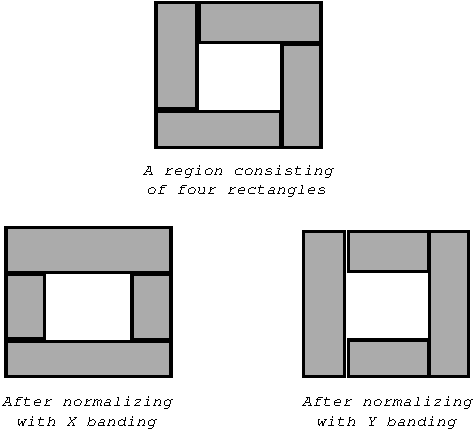
\includegraphics{region-normalization}}
\caption{Normalization of rectangular region sets.}
\end{figure}


\Defgeneric {region-union} {region1 region2}

Returns a region that contains all points that are in either of the
\term{regions} \arg{region1} or \arg{region2} (possibly with some points removed
in order to satisfy the dimensionality rule).  The result of \cl{region-union}
always has dimensionality that is the maximum dimensionality of \arg{region1}
and \arg{region2}.  For example, the union of a path and an area produces an
area; the union of two paths is a path.

\cl{region-union} will return either a simple region, a region set, or a member
of the class \cl{standard-region-union}.

\MayCaptureInputs

\Defgeneric {region-intersection} {region1 region2}

Returns a region that contains all points that are in both of the \term{regions}
\arg{region1} and \arg{region2} (possibly with some points removed in order to
satisfy the dimensionality rule).  The result of \cl{region-intersection} has
dimensionality that is the minimum dimensionality of \arg{region1} and
\arg{region2}, or is \cl{+nowhere+}.  For example, the intersection of two areas
is either another area or \cl{+nowhere+}; the intersection of two paths is
either another path or \cl{+nowhere+}; the intersection of a path and an area
produces the path clipped to stay inside of the area.

\cl{region-intersection} will return either a simple region or a member of the
class \cl{standard-region-intersection}.

\MayCaptureInputs

\Defgeneric {region-difference} {region1 region2}

Returns a region that contains all points in the \term{region} \arg{region1}
that are not in the \term{region} \arg{region2} (possibly plus additional
boundary points to make the result closed).  The result of
\cl{region-difference} has the same dimensionality as \arg{region1}, or is
\cl{+nowhere+}.  For example, the difference of an area and a path produces the
same area; the difference of a path and an area produces the path clipped to
stay outside of the area.

\cl{region-difference} will return either a simple region, a region set, or a
member of the class \cl{standard-region-difference}.

\MayCaptureInputs


\begin{figure}
\centerline{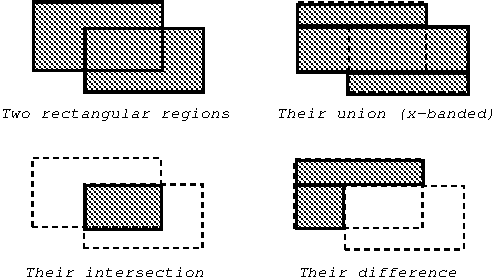
\includegraphics{region-composition}}
\caption{Examples of region union, intersection, and difference.}
\end{figure}


\section {Other Region Types}

The other types of regions are points, polylines, polygons, elliptical arcs, and
ellipses.  All of these region types are closed under affine transformations.

\Issue {SWM, York} {There is a proposal to remove the \cl{polygon},
\cl{polyline}, \cl{line}, \cl{ellipse}, and \cl{elliptical-arc} classes, since
they are only of limited utility, and CLIM itself doesn't use the classes at
all.  The advantage of removing these classes is that both the spec and CLIM
itself become a little simpler, and there are fewer cases of the region protocol
to implement.  However, removing these classes results in a geometric model that
is no longer closed (in the mathematical sense).  This lack of closure makes it
difficult to specify the design-based drawing model.  Furthermore, these are
intuitive objects that are used by a small, but important, class of
applications, and some people feel that CLIM should relieve programmers from
having to implement these classes for himself or herself.

The advocates of of removing these classes also propose removing the
design-based drawing model.  In this case, a more consistent proposal is to
remove all of the geometric classes, including \cl{point} and \cl{rectangle}.

Again, the opposing point of view believes that the power and flexibility of the
design-based drawing model does not justify the removal of any of these classes.
One counter-proposal is to require CLIM not to use any of the extended region
classes internally, and to move the implementation of the extended region
classes to a separately loadable module (via \cl{provide} and \cl{require}).}

\begin{figure}
\centerline{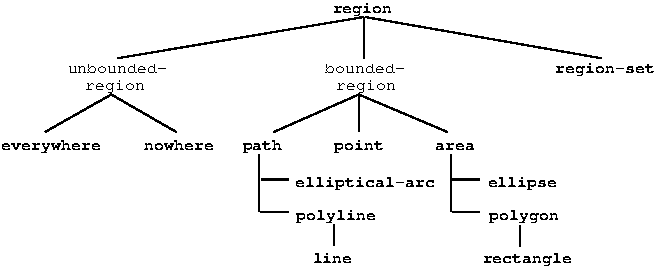
\includegraphics{region-structure}}
\caption{The class structure for all regions.}
\end{figure}


\subsection {Points}

A \concept{point} is a mathematical point in the plane, designated by its
coordinates, which are a pair of real numbers (where a real number is defined as
either an integer, a ratio, or a floating point number).  Points have neither
area nor length (that is, they have dimensionality 0).

Note well that a point is {\sl not} a pixel; CLIM models a drawing plane with
continuous coordinates.  This is discussed in more detail in
Chapter~\ref{graphics}.

\Defprotoclass {point}

The protocol class that corresponds to a mathematical point.  This is a subclass
of \cl{region} and \cl{bounding-rectangle}.
\IfYouWantClass {a} {point} {point}

\Defpredicate {pointp} {object}

Returns \term{true} if \arg{object} is a \term{point}, otherwise returns
\term{false}.

\Defclass {standard-point}

An instantiable class that implements a point.  This is a subclass of \cl{point}.
This is the class that \cl{make-point} instantiates.  
\Immutable

\Defun {make-point} {x y}

Returns an object of class \cl{standard-point} whose coordinates are \arg{x} and
\arg{y}.  \arg{x} and \arg{y} must be real numbers.


\subsubsection {The Point Protocol}

The following generic functions comprise the point API.  Only
\cl{point-position} is in the point protocol, that is, all classes that are
subclasses of \cl{point} must implement methods for \cl{point-position}, but
need not implement methods for \cl{point-x} and \cl{point-y}.

\Defgeneric {point-position} {point}

Returns both the $x$ and $y$ coordinates of the point \arg{point} as two values.

\defgeneric {point-x} {point}
\Defgeneric {point-y} {point}

Returns the $x$ or $y$ coordinate of the \term{point} \arg{point}, respectively.
CLIM will supply default methods for \cl{point-x} and \cl{point-y} on the
protocol class \cl{point} that are implemented by calling \cl{point-position}.


\subsection {Polygons and Polylines}

A \concept{polyline} is a path that consists of one or more line segments joined
consecutively at their end-points.

Polylines that have the end-point of their last line segment coincident with the
start-point of their first line segment are called \concept{closed}; this use of
the term ``closed'' should not be confused with closed sets of points.

A \concept{polygon} is an area bounded by a closed polyline. 

If the boundary of a polygon intersects itself, the odd-even winding-rule
defines the polygon: a point is inside the polygon if a ray from the point to
infinity crosses the boundary an odd number of times.

\Defprotoclass {polyline}

The protocol class that corresponds to a polyline.  This is a subclass of
\cl{path}.
\IfYouWantClass {a} {polyline} {polyline}

\Defpredicate {polylinep} {object}

Returns \term{true} if \arg{object} is a \term{polyline}, otherwise returns
\term{false}.

\Defclass {standard-polyline}

An instantiable class that implements a polyline.  This is a subclass of
\cl{polyline}.  This is the class that \cl{make-polyline} and
\cl{make-polyline*} instantiate.
\Immutable

\defun {make-polyline}  {point-seq \key closed}
\Defun {make-polyline*} {coord-seq \key closed}

Returns an object of class \cl{standard-polyline} consisting of the segments
connecting each of the points in \arg{point-seq} (or the points represented by
the coordinate pairs in \arg{coord-seq}).  \arg{point-seq} is a sequence of
\term{points}; \arg{coord-seq} is a sequence of coordinate pairs, which are real
numbers.  It is an error if \arg{coord-seq} does not contain an even number of
elements.

If \arg{closed} is \term{true}, then the segment connecting the first point and
the last point is included in the polyline.  The default for \arg{closed} is
\term{false}.

\MayCaptureInputs


\Defprotoclass {polygon}

The protocol class that corresponds to a mathematical polygon.  This is a
subclass of \cl{area}.
\IfYouWantClass {a} {polygon} {polygon}

\Defpredicate {polygonp} {object}

Returns \term{true} if \arg{object} is a \term{polygon}, otherwise returns
\term{false}.

\Defclass {standard-polygon}

An instantiable class that implements a polygon.  This is a subclass of
\cl{polygon}.  This is the class that \cl{make-polygon} and \cl{make-polygon*}
instantiate.
\Immutable

\defun {make-polygon}  {point-seq}
\Defun {make-polygon*} {coord-seq}

Returns an object of class \cl{standard-polygon} consisting of the area
contained in the boundary that is specified by the segments connecting each of
the points in \arg{point-seq} (or the points represented by the coordinate pairs
in \arg{coord-seq}).  \arg{point-seq} is a sequence of \term{points};
\arg{coord-seq} is a sequence of coordinate pairs, which are real numbers.  It
is an error if \arg{coord-seq} does not contain an even number of elements.

\MayCaptureInputs


\subsubsection {The Polygon and Polyline Protocol}

The following generic functions comprise the polygon and polyline protocol.  All
classes that are subclasses of either \cl{polygon} or \cl{polyline} must
implement methods for these generic functions.  Some of the functions below take
an argument named \arg{polygon-or-polyline}; this argument may be either a
\term{polygon} or a \term{polyline}.

\Defgeneric {polygon-points} {polygon-or-polyline}

Returns a sequence of points that specify the segments in \arg{polygon-or-polyline}.
\ReadOnly

\Defgeneric {map-over-polygon-coordinates} {function polygon-or-polyline}

Applies \arg{function} to all of the coordinates of the vertices of
\arg{polygon-or-polyline}.  \arg{function} is a function of two arguments, the
$x$ and $y$ coordinates of the vertex; it has dynamic extent.

\Defgeneric {map-over-polygon-segments} {function polygon-or-polyline}

Applies \arg{function} to the segments that compose \arg{polygon-or-polyline}.
\arg{function} is a function of four arguments, the $x$ and $y$ coordinates of
the start of the segment, and the $x$ and $y$ coordinates of the end of the
segment; it has dynamic extent.  When \cl{map-over-polygon-segments} is called
on a closed polyline, it will call \arg{function} on the segment that connects
the last point back to the first point.

\Defgeneric {polyline-closed} {polyline}

Returns \term{true} if the polyline \arg{polyline} is closed, otherwise returns
\term{false}.  This function need be implemented only for \term{polylines}, not
for \term{polygons}.


\subsection {Lines}

A line is a polyline consisting of a single segment.

\Defprotoclass {line}

The protocol class that corresponds to a mathematical line segment, that is, a
polyline with only a single segment.  This is a subclass of \cl{polyline}.
\IfYouWantClass {a} {line} {line}

\Defpredicate {linep} {object}

Returns \term{true} if \arg{object} is a \term{line}, otherwise returns
\term{false}.

\Defclass {standard-line}

An instantiable class that implements a line segment.  This is a subclass of
\cl{line}.  This is the class that \cl{make-line} and \cl{make-line*}
instantiate.
\Immutable

\defun {make-line}  {start-point end-point}
\Defun {make-line*} {start-x start-y end-x end-y}

Returns an object of class \cl{standard-line} that connects the two
\term{points} \arg{start-point} and \arg{end-point} (or the positions
(\arg{start-x},\arg{start-y}) and (\arg{end-x},\arg{end-y})).

\MayCaptureInputs


\subsubsection {The Line Protocol}

The following generic functions comprise the line API.  Only
\cl{line-start-point*} and \cl{line-end-point*} are in the line protocol, that
is, all classes that are subclasses of \cl{line} must implement methods for
\cl{line-start-point*} and \cl{line-end-point*}, but need not implement methods
for \cl{line-start-point} and \cl{line-end-point}.

\defgeneric {line-start-point*} {line}
\Defgeneric {line-end-point*}   {line}

Returns the starting or ending point, respectively, of the \term{line}
\arg{line} as two real numbers representing the coordinates of the point.

\defgeneric {line-start-point} {line}
\Defgeneric {line-end-point}   {line}

Returns the starting or ending point of the \term{line} \arg{line},
respectively.

CLIM will supply default methods for \cl{line-start-point} and
\cl{line-end-point} on the protocol class \cl{line} that are implemented by
calling \cl{line-start-point*} and \cl{line-end-point*}.


\subsection {Rectangles} 
\label {rect}

Rectangles whose edges are parallel to the coordinate axes are a special case of
polygon that can be specified completely by four real numbers
(\arg{x1},\arg{y1},\arg{x2},\arg{y2}).  They are {\sl not} closed under general
affine transformations (although they are closed under rectilinear
transformations).

\Defprotoclass {rectangle}

The protocol class that corresponds to a mathematical rectangle, that is,
rectangular polygons whose sides are parallel to the coordinate axes.  This is a
subclass of \cl{polygon}.
\IfYouWantClass {a} {rectangle} {rectangle}

\Defpredicate {rectanglep} {object}

Returns \term{true} if \arg{object} is a \term{rectangle}, otherwise returns
\term{false}.

\Defclass {standard-rectangle}

An instantiable class that implements an axis-aligned rectangle.  This is a
subclass of \cl{rectangle}.  This is the class that \cl{make-rectangle} and
\cl{make-rectangle*} instantiate.
\Immutable

\defun {make-rectangle}  {point1 point2}
\Defun {make-rectangle*} {x1 y1 x2 y2}

Returns an object of class \cl{standard-rectangle} whose edges are parallel to
the coordinate axes.  One corner is at the \term{point} \arg{point1} (or the
position (\arg{x1},\arg{y1})) and the opposite corner is at the \term{point}
\arg{point2} (or the position (\arg{x2},\arg{y2})).  There are no ordering
constraints among \arg{point1} and \arg{point2} (or \arg{x1} and \arg{x2}, and
\arg{y1} and \arg{y2}).

Most CLIM implementations will choose to represent rectangles in the most
efficient way, such as by storing the coordinates of two opposing corners of the
rectangle.  Because this representation is not sufficient to represent the
result of arbitrary transformations of arbitrary rectangles, CLIM is allowed to
return a polygon as the result of such a transformation.  (The most general
class of transformations that is guaranteed to always turn a rectangle into
another rectangle is the class of transformations that satisfy
\cl{rectilinear-transformation-p}.)

\MayCaptureInputs


\subsubsection {The Rectangle Protocol}

The following generic functions comprise the rectangle API.  Only
\cl{rectangle-edges*} is in the rectangle protocol, that is, all classes that
are subclasses of \cl{rectangle} must implement methods for
\cl{rectangle-edges*}, but need not implement methods for the remaining
functions.

\Defgeneric {rectangle-edges*} {rectangle}

Returns the coordinates of the minimum $x$ and $y$ and maximum $x$ and $y$ of
the rectangle \arg{rectangle} as four values, \arg{min-x}, \arg{min-y},
\arg{max-x}, and \arg{max-y}.

\defgeneric {rectangle-min-point} {rectangle}
\Defgeneric {rectangle-max-point} {rectangle}

Returns the min point and max point of the \term{rectangle} \arg{rectangle},
respectively.  The position of a rectangle is specified by its min point.

CLIM will supply default methods for \cl{rectangle-min-point} and
\cl{rectangle-max-point} on the protocol class \cl{rectangle} that are
implemented by calling \cl{rectangle-edges*}.


\defgeneric {rectangle-min-x} {rectangle}
\defgeneric {rectangle-min-y} {rectangle}
\defgeneric {rectangle-max-x} {rectangle}
\Defgeneric {rectangle-max-y} {rectangle}

Returns (respectively) the minimum $x$ and $y$ coordinate and maximum $x$ and
$y$ coordinate of the \term{rectangle} \arg{rectangle}.

CLIM will supply default methods for these four generic functions on the
protocol class \cl{rectangle} that are implemented by calling
\cl{rectangle-edges*}.


\defgeneric {rectangle-width}  {rectangle}
\defgeneric {rectangle-height} {rectangle}
\Defgeneric {rectangle-size}   {rectangle}

\cl{rectangle-width} returns the width of the \term{rectangle} \arg{rectangle},
which is the difference between the maximum $x$ and its minimum $x$.
\cl{rectangle-height} returns the height, which is the difference between the
maximum $y$ and its minimum $y$.  \cl{rectangle-size} returns two values, the
width and the height.

CLIM will supply default methods for these four generic functions on the
protocol class \cl{rectangle} that are implemented by calling
\cl{rectangle-edges*}.


\subsection {Ellipses and Elliptical Arcs}

An \concept{ellipse} is an area that is the outline and interior of an ellipse.
Circles are special cases of ellipses.

An \concept{elliptical arc} is a path consisting of all or a portion of the
outline of an ellipse.  Circular arcs are special cases of elliptical arcs.

An ellipse is specified in a manner that is easy to transform, and treats all
ellipses on an equal basis.  An ellipse is specified by its center point and two
vectors that describe a bounding parallelogram of the ellipse.  The bounding
parallelogram is made by adding and subtracting the vectors from the the center
point in the following manner:

\begin{tabular}{|c|cc|}
 \hline
   & {\sl $x$ coordinate} & {\sl $y$ coordinate} \\
 \hline
 Center of Ellipse & $x_c$ & $y_c$ \\
 \hline
 Vectors & $dx_1$ & $dy_1$ \\
         & $dx_2$ & $dy_2$ \\
 \hline
 Corners of Parallelogram & $x_c + dx_1 + dx_2$ & $y_c + dy_1 + dy_2$ \\
                          & $x_c + dx_1 - dx_2$ & $y_c + dy_1 - dy_2$ \\
                          & $x_c - dx_1 - dx_2$ & $y_c - dy_1 - dy_2$ \\
                          & $x_c - dx_1 + dx_2$ & $y_c - dy_1 + dy_2$ \\
 \hline
\end{tabular}

Note that several different parallelograms specify the same ellipse.  One
parallelogram is bound to be a rectangle---the vectors will be perpendicular
and correspond to the semi-axes of the ellipse.

\begin{figure}
\centerline{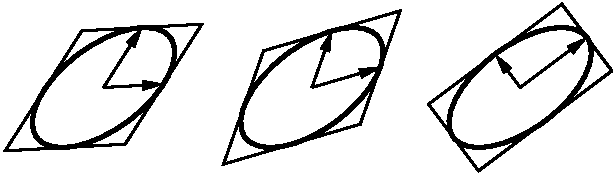
\includegraphics{different-ellipses}}
\caption{Different vectors may specify the same ellipse.}
\end{figure}

The special case of an ellipse with its axes aligned with the coordinate axes
can be obtained by setting $dx_2 = dy_1 = 0$ or $dx_1 = dy_2 = 0$.


\Defprotoclass {ellipse}

The protocol class that corresponds to a mathematical ellipse.  This is a
subclass of \cl{area}.
\IfYouWantClass {an} {ellipse} {ellipse}

\Defpredicate {ellipsep} {object}

Returns \term{true} if \arg{object} is an \term{ellipse}, otherwise returns
\term{false}.

\Defclass {standard-ellipse}

An instantiable class that implements an ellipse.  This is a subclass of
\cl{ellipse}.  This is the class that \cl{make-ellipse} and \cl{make-ellipse*}
instantiate.
\Immutable

\defun {make-ellipse}  {center-point 
                        radius-1-dx radius-1-dy radius-2-dx radius-2-dy
                        \key start-angle end-angle}
\Defun {make-ellipse*} {center-x center-y 
                        radius-1-dx radius-1-dy radius-2-dx radius-2-dy 
                        \key start-angle end-angle}

Returns an object of class \cl{standard-ellipse}.  The center of the ellipse is
at the \term{point} \arg{center-point} (or the position
(\arg{center-x},\arg{center-y})).

Two vectors, (\arg{radius-1-dx},\arg{radius-1-dy}) and
(\arg{radius-2-dx},\arg{radius-2-dy}) specify the bounding parallelogram of the
ellipse as explained above.  All of the radii are real numbers.  If the two
vectors are collinear, the ellipse is not well-defined and the
\cl{ellipse-not-well-defined} error will be signalled.  The special case of an
ellipse with its axes aligned with the coordinate axes can be obtained by
setting both \arg{radius-1-dy} and \arg{radius-2-dx} to 0.

If \arg{start-angle} or \arg{end-angle} are supplied, the ellipse is the ``pie
slice'' area swept out by a line from the center of the ellipse to a point on
the boundary as the boundary point moves from the angle \arg{start-angle} to
\arg{end-angle}.  Angles are measured counter-clockwise with respect to the
positive $x$ axis.  If \arg{end-angle} is supplied, the default for
\arg{start-angle} is $0$; if \arg{start-angle} is supplied, the default for
\arg{end-angle} is $2\pi$; if neither is supplied then the region is a full
ellipse and the angles are meaningless.

\MayCaptureInputs


\Defprotoclass {elliptical-arc}

The protocol class that corresponds to a mathematical elliptical arc.  This is a
subclass of \cl{path}.
\IfYouWantClass {an} {elliptical arc} {elliptical-arc}

\Defpredicate {elliptical-arc-p} {object}

Returns \term{true} if \arg{object} is an \term{elliptical arc}, otherwise
returns \term{false}.

\Defclass {standard-elliptical-arc}

An instantiable class that implements an elliptical arc.  This is a subclass of
\cl{elliptical-arc}.  This is the class that \cl{make-elliptical-arc} and
\cl{make-elliptical-arc*} instantiate.
\Immutable

\defun {make-elliptical-arc}  {center-point
                               radius-1-dx radius-1-dy radius-2-dx radius-2-dy
                               \key start-angle end-angle}
\Defun {make-elliptical-arc*} {center-x center-y 
                               radius-1-dx radius-1-dy radius-2-dx radius-2-dy
                               \key start-angle end-angle}

Returns an object of class \cl{standard-elliptical-arc}.  The center of the
ellipse is at the \term{point} \arg{center-point} (or the position
(\arg{center-x},\arg{center-y})).

Two vectors, (\arg{radius-1-dx},\arg{radius-1-dy}) and
(\arg{radius-2-dx},\arg{radius-2-dy}), specify the bounding parallelogram of the
ellipse as explained above.  All of the radii are real numbers.   If the two
vectors are collinear, the ellipse is not well-defined and the
\cl{ellipse-not-well-defined} error will be signalled.  The special case of
an elliptical arc with its axes aligned with the coordinate axes can be obtained
by setting both \arg{radius-1-dy} and \arg{radius-2-dx} to 0.

If \arg{start-angle} and \arg{start-angle} are supplied, the arc is swept from
\arg{start-angle} to \arg{end-angle}.  Angles are measured counter-clockwise
with respect to the positive $x$ axis.  If \arg{end-angle} is supplied, the
default for \arg{start-angle} is $0$; if \arg{start-angle} is supplied, the
default for \arg{end-angle} is $2\pi$; if neither is supplied then the region is
a closed elliptical path and the angles are meaningless.

\MayCaptureInputs


\subsubsection {The Ellipse and Elliptical Arc Protocol}

The following functions apply to both ellipses and elliptical arcs.  In all
cases, the name \arg{elliptical-object} means that the argument may be an
\term{ellipse} or an \term{elliptical arc}.  These generic functions comprise
the ellipse protocol.  All classes that are subclasses of either \cl{ellipse} or
\cl{elliptical-arc} must implement methods for these functions.

\Defgeneric {ellipse-center-point*} {elliptical-object}

Returns the center point of \arg{elliptical-object} as two values representing
the coordinate pair.

\Defgeneric {ellipse-center-point} {elliptical-object}

Returns the center point of \arg{elliptical-object}.  

\cl{ellipse-center-point} is part of the ellipse API, but not part of the ellipse
protocol.  CLIM will supply default methods for \cl{ellipse-center-point} on the
protocol classes \cl{ellipse} and \cl{elliptical-arc} that are implemented by
calling \cl{ellipse-center-point*}.

\Defgeneric {ellipse-radii} {elliptical-object}

Returns four values corresponding to the two radius vectors of
\arg{elliptical-arc}.  These values may be canonicalized in some way, and so may
not be the same as the values passed to the constructor function.

\Defgeneric {ellipse-start-angle} {elliptical-object}

Returns the start angle of \arg{elliptical-object}.  If \arg{elliptical-object}
is a full ellipse or closed path then \cl{ellipse-start-angle} will return
\cl{nil}; otherwise the value will be a number greater than or equal to zero,
and less than $2\pi$.

\Defgeneric {ellipse-end-angle} {elliptical-object}

Returns the end angle of \arg{elliptical-object}.  If \arg{elliptical-object} is
a full ellipse or closed path then \cl{ellipse-end-angle} will return \cl{nil};
otherwise the value will be a number greater than zero, and less than or equal
to $2\pi$.

